\documentclass[11pt,a4paper]{article}
\usepackage[utf8]{inputenc}
\usepackage[T1]{fontenc}
\usepackage{amsmath}
\usepackage{amsfonts}
\usepackage{amssymb}
\usepackage{graphicx}
\usepackage{booktabs}
\usepackage{array}
\usepackage{hyperref}
\usepackage{cite}
\usepackage{geometry}
\usepackage{enumitem}
\geometry{margin=1in}
\usepackage{longtable}

\title{ATLAS Final Project Report\\
Adaptive Task-Aware Federated Learning with Heterogeneous LoRA\\
and Split Learning for Edge LLMs}

\author{%
Mahmoud Mayaleh\\[6pt]
{\small Prof.\ Lyes Khoukhi (CNAM, France)}\\
{\small Zakaria Abou El Houda (INRS, Canada)}
}
\date{February 23, 2026}

\begin{document}

\maketitle

\tableofcontents
\newpage


\section{Base Specifications}

Large language models (LLMs) have revolutionized natural language processing, but their deployment and fine-tuning remain computationally prohibitive for resource-constrained edge devices. Traditional federated learning approaches either require substantial on-device computation or fail to accommodate the heterogeneity inherent in real-world distributed systems. This project addresses these limitations by developing a heterogeneous Split-LoRA framework that enables collaborative model training across devices with dramatically different computational capabilities.

The primary objective is to design and implement a federated learning system that combines split learning and parameter-efficient fine-tuning (PEFT) to enable resource-constrained devices to participate meaningfully in collaborative model training. Specific goals include: (1) design a split learning architecture that partitions transformer models between client and server, minimizing client-side computational requirements; (2) implement device-aware heterogeneous LoRA configurations that assign different low-rank adaptation parameters based on device capabilities; (3) develop federated aggregation mechanisms that handle heterogeneous model updates from clients with different LoRA ranks; (4) validate the framework on classification tasks using standard NLP benchmarks; and (5) quantify memory--accuracy trade-offs across device profiles.

The implementation encompasses three major components. First, a LoRA adapter module implementing low-rank matrix factorization, following Hu et al. (2021). Second, a split learning architecture that divides transformer layers, with clients computing activations through frozen bottom layers and trainable LoRA adapters, and the server processing top layers with a classification head. Third, a heterogeneous federated aggregation system implementing device-specific aggregation that groups clients by device type and aggregates within groups to prevent tensor dimension mismatches.

The validation framework employs multiple backbones spanning encoder and decoder architectures. Evaluation metrics include validation accuracy (or F1/Matthews correlation as appropriate), client-side memory footprint, communication costs, and convergence behavior.

\section{Development Plan}

\subsection{Original Plan (Mid-Term)}

The project was originally structured into four sequential tasks spanning November 2025 to February 2026:

\begin{itemize}
\item \textbf{Task 1 --- State of the Art Review} (Nov 17 -- Dec 19, 2025, 5 weeks): Literature survey on transformers, GPT-2, federated learning, split learning, and PEFT methods. \emph{Status at mid-term: Completed.}
\item \textbf{Task 2 --- Designing Optimized Split-LoRA Framework} (Dec 22, 2025 -- Jan 30, 2026, 6 weeks): Implementation of the core heterogeneous Split-LoRA framework including LoRA adapter modules, split client/server components, and device-aware aggregation. \emph{Status at mid-term: In progress (\textasciitilde70\%).}
\item \textbf{Task 3 --- Testing, Evaluation, and Extensions} (Feb 2 -- Feb 13, 2026, 2 weeks): Full-scale experiments, ablation studies, and additional scenarios. \emph{Status at mid-term: Planned.}
\item \textbf{Task 4 --- Writing, Documentation, and Reproducibility} (Feb 16 -- Feb 20, 2026, 1 week): Report finalization, code documentation, and reproducibility bundle. \emph{Status at mid-term: Planned.}
\end{itemize}

\subsection{Applied Changes and Revised Plan}

The scope of the project expanded, and the key changes are:

\begin{enumerate}
\item \textbf{Expanded problem formulation}: The project evolved from a heterogeneous Split-LoRA baseline (GPT-2 + SST-2, 4 clients, phone/edge/GPU profiles) into a full task-aware federated multi-task learning framework named \textbf{ATLAS}. This expansion was motivated by insights from the literature review revealing that task-agnostic global aggregation causes negative transfer in multi-task settings.

\item \textbf{Multi-backbone evaluation}: Instead of a single GPT-2 model, the evaluation now covers three backbones (DistilBERT-base-uncased, GPT-2, and Qwen2.5), spanning encoder and decoder architectures.

\item \textbf{Multi-task GLUE evaluation}: The experimental protocol expanded from SST-2 only to four GLUE tasks (SST-2, MRPC, CoLA, QNLI) with 12 clients (3 per task), enabling genuine multi-task federation.

\item \textbf{Four-phase ATLAS pipeline}: The framework now integrates (i) gradient-based task clustering via compact fingerprints, (ii) device-aware heterogeneous LoRA rank allocation under explicit memory budgets, (iii) split federated learning with adaptive split selection and per-cluster aggregation, and (iv) MIRA-style Laplacian regularization over an RBF-kernel task graph.
\end{enumerate}


\section{State of the Art}

\subsection{Parameter-Efficient Fine-Tuning (PEFT)}

Full fine-tuning of large pre-trained models is computationally expensive and requires storing complete model copies for each downstream task. Parameter-efficient fine-tuning methods address this by updating only a small subset of parameters while keeping the pre-trained weights frozen.

\paragraph{Low-Rank Adaptation (LoRA).}
Hu et al. (2021) introduced LoRA, a reparameterization-based PEFT method that factorizes weight updates into low-rank matrices. For a pre-trained weight matrix $W_0 \in \mathbb{R}^{d\times d}$, LoRA represents the update as $\Delta W = BA$ where $B \in \mathbb{R}^{d\times r}$ and $A \in \mathbb{R}^{r\times d}$ with rank $r \ll d$. During training, $W_0$ remains frozen while only $A$ and $B$ are optimized, reducing trainable parameters from $d^2$ to $2dr$. Hu et al. demonstrate that LoRA matches or exceeds full fine-tuning performance on RoBERTa and GPT-3 while using orders of magnitude fewer trainable parameters. The success stems from the hypothesis that task-specific adaptations lie in low-dimensional subspaces, validated empirically across multiple model scales.

\paragraph{Adapter Modules.}
Houlsby et al. (2019) pioneered adapter-based PEFT by inserting small bottleneck modules into each transformer layer. An adapter module consists of a down-projection, a non-linearity, an up-projection, and a residual connection. Pfeiffer et al. (2020) demonstrated that inserting adapters only after the feed-forward layers achieves comparable performance with 50\% fewer parameters. The modular nature of adapters enables task composition through AdapterFusion for multi-task learning scenarios.

\subsection{Federated Learning Foundations}

Federated learning (FL), formalized by McMahan et al. (2017), enables collaborative model training across distributed clients without centralizing raw data. The Federated Averaging (FedAvg) algorithm proceeds iteratively: the server broadcasts the global model, clients train locally, and the server aggregates updates through weighted averaging. Real-world FL faces three fundamental challenges: data heterogeneity from non-i.i.d.\ distributions, system heterogeneity from varying device capabilities, and communication efficiency as model sizes grow.

\subsection{Split Learning for LLMs}

Split learning partitions neural networks between clients and a server, with clients computing only through the cut layer before transmitting activations. This dramatically reduces client-side computational requirements. Vepakomma et al. (2018) demonstrated that split learning achieves comparable accuracy to centralized training while requiring 45\% less client-side computation than federated learning.

\paragraph{SplitLoRA and HSplitLoRA.}
Lin et al. (2024) proposed SplitLoRA, integrating split learning with LoRA adapters for LLM fine-tuning. The subsequent HSplitLoRA framework (Lin et al., 2025) extends this to heterogeneous settings through three key innovations: (a) an important weight identification scheme based on resource-normalized gradient-weight product (RNGWP) to prioritize trainable weights; (b) adaptive rank and model splitting configuration that dynamically adjusts decomposition ranks and the model split point to match heterogeneous computing budgets; and (c) a noise-free adapter aggregation mechanism that concatenates low-rank decomposition matrices rather than averaging them, achieving mathematically consistent aggregation without introducing noise. Extensive experiments on LLaMA-2-7B and GPT-2-L demonstrate that HSplitLoRA outperforms state-of-the-art benchmarks in training accuracy and convergence speed under both homogeneous and heterogeneous settings.

\subsection{Federated PEFT and Heterogeneous Configurations}

\paragraph{FAH-QLoRA.}
Gao et al. (2025) proposed FAH-QLoRA, a federated adaptive fine-tuning framework that combines heterogeneous model quantization with adaptive LoRA ranks. The framework dynamically adjusts LoRA ranks across training rounds to promote faster convergence and assigns heterogeneous ranks across devices to mitigate the straggler effect. A two-stage approach first optimizes the average LoRA rank by maximizing the loss decrease rate, then assigns device-specific ranks via a convex optimization formulation. Experiments show that FAH-QLoRA reduces training time by up to 45.86\% and memory usage by up to 44.15\% compared to baselines while maintaining comparable accuracy. The convergence is proven under non-convex and non-i.i.d.\ settings, providing theoretical guarantees for heterogeneous rank deployment.

\paragraph{HetLoRA and FlexLoRA.}
Cho et al. (2023) introduced HetLoRA, demonstrating that heterogeneous LoRA ranks in FL can optimize performance while minimizing communication rounds. FlexLoRA (Bai et al., 2024) extends this through SVD-based weight redistribution, dynamically adjusting local LoRA ranks and achieving 3.2\% higher accuracy than truncation-based aggregation.

\subsection{Federated Multi-Task Learning}

\paragraph{MIRA.}
Elbakary et al. (2025) introduced MIRA, a federated multi-task learning method for LLMs that leverages Laplacian regularization over a task-similarity graph to enable client-specific personalization while maintaining global coherence. The FMTL objective minimizes a global loss augmented by a Laplacian regularization term
\[
R(W) = W^\top \tilde{L} W = \frac{1}{2}\sum_k\sum_l a_{kl}\|w_k - w_l\|^2,
\]
where $a_{kl}$ quantifies inter-task similarity. MIRA uses LoRA for efficiency and performs server-side regularization updates after local training. Experiments on Data-Juicer (1.3B) and GPT-2-large with Natural Instructions and Dolly-15k datasets show that MIRA achieves lower per-task loss than FedIT and FedPTuning while maintaining comparable global performance.

\subsection{Positioning of ATLAS}

Existing methods address individual aspects --- FMTL (MIRA), heterogeneous PEFT (FAH-QLoRA, HetLoRA), and split execution (SplitLoRA, HSplitLoRA) --- largely in isolation. None jointly integrates automatic task discovery, device-aware heterogeneous adapter allocation, split execution under memory constraints, and graph-based personalization into a single pipeline. ATLAS fills this gap by coupling gradient-based task clustering, importance-guided heterogeneous LoRA rank allocation under explicit budgets, heuristic-driven split selection, and MIRA-style Laplacian regularization over fingerprint-derived task graphs.

\begin{center}
\begin{tabular}{lcccc}
\toprule
\textbf{Work} & \textbf{Task-Aware} & \textbf{Het. PEFT} & \textbf{Split} & \textbf{Graph Reg.}\\
\midrule
MIRA & $\checkmark$ & $\times$ & $\times$ & $\checkmark$\\
FAH-QLoRA & $\times$ & $\checkmark$ & $\times$ & $\times$\\
HSplitLoRA & $\times$ & $\checkmark$ & $\checkmark$ & $\times$\\
\textbf{ATLAS (this work)} & $\checkmark$ & $\checkmark$ & $\checkmark$ & $\checkmark$\\
\bottomrule
\end{tabular}
\end{center}


\section{Analysis}

\subsection{Problem Decomposition}

The ATLAS framework addresses a coupled optimization problem spanning four dimensions: task structure discovery, resource-constrained adapter allocation, split-point selection, and inter-client personalization.

\paragraph{Task Heterogeneity and Negative Transfer.}
In multi-task federation, naively averaging updates across clients solving different NLP tasks (e.g., sentiment analysis, paraphrase detection, grammatical acceptability, question answering) causes negative transfer --- updates from one task degrade performance on another. MIRA's experiments show that global model performance varies significantly across tasks, with the global model performing worse than local-only training in certain tasks. ATLAS addresses this through gradient-based task clustering (Phase 1), which discovers task structure without sharing labels or raw data.

\paragraph{Device Heterogeneity and Memory Constraints.}
Edge devices exhibit strong variation in memory (2--16 GB GPU budgets in the experimental federation). Uniform-rank LoRA configurations either exceed low-end device capacity or underutilize high-end devices. HSplitLoRA demonstrated that the device unavailability problem degrades converged accuracy by 0.23 PPL and slows convergence by 42\% on LLaMA-2-7B as the unavailability rate increases from 0\% to 50\%. FAH-QLoRA showed that heterogeneous rank assignment combined with quantization reduces training time by up to 45.86\%. ATLAS extends this by allocating per-layer ranks from discrete candidates under explicit per-device memory budgets, using importance signals from gradient statistics (Phase 2).

\paragraph{Split-Point Selection.}
The model split point determines the distribution of computing load between client and server. HSplitLoRA's measurements show that model split point trades off client-side and server-side computing overhead while affecting training performance. ATLAS formalizes this through a heuristic weighted-score split selector combining memory feasibility, communication cost, importance proxy, and workload balance terms (Phase 3).

\paragraph{Personalization vs.\ Collaboration.}
Pure local training maximizes personalization but forgoes cross-client knowledge transfer, especially harmful when local data is scarce. Pure global averaging maximizes collaboration but sacrifices task-specific adaptation. MIRA's Laplacian regularization provides a principled middle ground, and ATLAS adapts this to LoRA-only personalization with fingerprint-derived RBF-kernel graphs and block-diagonal structure enforced by cluster assignments (Phase 4).

\subsection{Functional Requirements}

The system satisfies the following updated functional requirements:

\begin{itemize}
\item \textbf{FR1 --- Multi-Backbone Split Architecture:} The system partitions pre-trained transformer models (DistilBERT, GPT-2, Qwen2.5) at configurable split layers. Clients compute activations through frozen prefix layers; the server completes forward propagation and backpropagation through suffix layers and task-specific classification heads.
\item \textbf{FR2 --- Importance-Guided Heterogeneous LoRA Allocation:} The system computes per-layer importance weights from gradient statistics and allocates LoRA ranks from discrete candidates \{4, 8, 16, 32, 64\} under explicit per-device memory budgets. The allocation uses an importance-aware, budget-constrained procedure that maximizes utilization on heterogeneous devices.
\item \textbf{FR3 --- Task-Aware Federated Aggregation:} The system implements per-cluster FedAvg aggregation (no cross-cluster averaging) based on Phase 1 cluster assignments, preventing negative transfer across tasks.
\item \textbf{FR4 --- Privacy-Preserving Communication:} Raw data never leaves client devices. Client-to-server communication transmits only intermediate activations; server-to-client transmits only activation gradients and aggregated LoRA parameters.
\item \textbf{FR5 --- Laplacian Personalization:} The system constructs a fingerprint-derived task graph and applies MIRA-style regularization to couple similar clients while preserving task-specific specialization.
\item \textbf{FR6 --- Comprehensive Evaluation:} The system evaluates across four GLUE tasks, three backbones, five ablation levels, and three random seeds, reporting task metrics, peak memory, communication volume, and convergence behavior.
\end{itemize}

\subsection{Design Constraints and Trade-offs}

Key design constraints include: (a) memory budget heterogeneity (2--16 GB) requires flexible rank allocation; (b) communication cost scales with activation size at the split point, favoring deeper splits for smaller activations but at the cost of increased client computation; (c) the Laplacian regularization strength $\eta$ trades off collaboration benefit against over-smoothing risk; and (d) the number of clusters trades off task-specific specialization (more clusters) against collaboration opportunities (fewer clusters).

\section{Realized and Implemented Design}

\subsection{System Architecture}

ATLAS is implemented as an end-to-end Python pipeline using PyTorch and HuggingFace Transformers. The architecture consists of four main modules corresponding to the four phases, orchestrated by a federated training loop.

\paragraph{Phase 1 --- Gradient Fingerprinting and Task Clustering.}
For each client $k$, ATLAS computes a compact gradient fingerprint by collecting gradients from task-relevant late layers and the classifier over a small number of mini-batches. Gradients are layer-wise normalized to prevent domination by large tensors, then projected to a fixed dimensionality of $d_f = 64$ via PCA. The system runs $k$-means over a constrained candidate range $[k_{\min}, k_{\max}]$ and selects $k^\star$ via a multi-metric score combining Silhouette, Davies-Bouldin, and Calinski-Harabasz indices with a singleton penalty term. The output is cluster assignments $c_k$ used in subsequent phases.

\paragraph{Phase 2 --- Device-Aware Heterogeneous LoRA Rank Allocation.}
Each client $k$ has a memory budget $M_k$. ATLAS reserves fractions for the frozen base model, activations, and optimizer state to derive an adapter budget $C_k^{adpt}$. Per-layer importance weights are derived from squared gradient norms aggregated during fingerprinting in Phase 1. The allocation algorithm finds the largest feasible uniform rank, converts it into a total rank budget, distributes proportionally to layer importance, rounds to valid candidates from the discrete set \{4, 8, 16, 32, 64\}, and downgrades least-important layers if needed to satisfy the budget constraint. This design draws on insights from HSplitLoRA's observation that different trainable weights contribute unequally to training performance and that weight importance varies throughout training.

\paragraph{Phase 3 --- Split Federated Learning with Heuristic Split Selection.}
ATLAS partitions the backbone at split layer $s$ into a client-side prefix and server-side suffix. The split is selected by minimizing a weighted score:
\[
\mathrm{Score}(s) = \alpha\cdot\mathrm{Mem}(s) + \beta\cdot\mathrm{Comm}(s) + \gamma\cdot\mathrm{Imp}(s) + \delta\cdot\mathrm{Bal}(s),
\]
where $\alpha$ controls emphasis on memory budget feasibility, $\beta$ penalizes communication-heavy splits, $\gamma$ weights an importance proxy from gradient fingerprints, and $\delta$ encourages balanced workload. Default weights are $\alpha=0.35$, $\beta=0.30$, $\gamma=0.25$, $\delta=0.10$, selected via preliminary sweeps. After local updates, per-cluster FedAvg aggregation is applied within each Phase-1 cluster only, with no cross-cluster averaging.

\paragraph{Phase 4 --- Laplacian Regularization over Task Graph.}
ATLAS constructs a task graph from fingerprints using RBF-kernel adjacency weights:
\[
a_{kl} = \exp\left(-\frac{\lVert f_k - f_l\rVert^2}{\sigma^2}\right),
\]
then row-normalized. Cross-cluster edges are removed and singletons are connected to $K_{nn}$ nearest neighbors for connectivity. The Laplacian update is:
\[
w_k \leftarrow w_k - \eta \sum_l a_{kl}(w_k - w_l),
\]
where $\eta$ controls coupling strength. This follows MIRA's server-side regularization approach but adapts it to LoRA-only parameters with fingerprint-derived graphs and block-diagonal cluster structure.

\subsection{Technology Stack}

\begin{center}
\begin{tabular}{ll}
\toprule
\textbf{Component} & \textbf{Technology}\\
\midrule
Deep learning framework & PyTorch 2.0+\\
Transformer models & HuggingFace Transformers\\
Data pipeline & HuggingFace Datasets (GLUE benchmark)\\
Optimization & AdamW with cosine annealing and warm-up\\
Precision & Mixed precision (fp16) where supported\\
Reproducibility & Fixed seeds (42, 123, 456), Python logging\\
\bottomrule
\end{tabular}
\end{center}

\subsection{Heterogeneous Rank Handling}

To align adapters across clients with varying ranks $r_k \neq r_l$, ATLAS supports three rank-alignment modes: \texttt{pad-to-max} (zero-padding to the maximum rank), \texttt{clip-to-min} (clipping to minimum rank), and \texttt{proj} (projection to a shared subspace). This is inspired by the zero-padding and truncation strategies employed in FAH-QLoRA and the noise-free concatenation approach of HSplitLoRA. The Laplacian runs server-side on per-cluster aggregated adapters, pre-global FedAvg.

\subsection{Mapping to Functional Requirements}

FR1 maps to the multi-backbone split architecture supporting DistilBERT, GPT-2, and Qwen2.5 with configurable split layers. FR2 maps to the Phase-2 importance-guided rank allocation algorithm. FR3 maps to the Phase-3 per-cluster FedAvg loop. FR4 maps to the activation-only communication protocol where only smashed data and gradients cross the network boundary. FR5 maps to the Phase-4 Laplacian regularization module. FR6 maps to the comprehensive experiment runner with multi-seed evaluation, metrics logging, and visualization.


\section{Evaluation, Experimentation, and Project Realization}

\subsection{Experimental Setup}

\paragraph{Tasks, Data, and Client Federation.}
ATLAS is evaluated in a heterogeneous multi-task FL setting using four GLUE sentence classification tasks: SST-2 (sentiment analysis), MRPC (paraphrase detection), CoLA (linguistic acceptability), and QNLI (question natural language inference). A federation of $K=12$ clients is simulated, with 3 clients per task and heterogeneous device profiles emulating 2--16 GB memory budgets. Each client uses up to 3,000 local training samples, subsampled if necessary to control runtime variance.

\paragraph{Models.}
Three backbones are considered: DistilBERT-base-uncased (encoder, \textasciitilde66M parameters), GPT-2 (decoder, \textasciitilde117M parameters), and Qwen2.5 (decoder, \textasciitilde500M parameters). This multi-backbone design tests ATLAS's generality across encoder and decoder architectures of varying scale.

\paragraph{Training Protocol.}
Federated training runs for 10 communication rounds with 3 local epochs per round. Each configuration is repeated with three independent seeds (42, 123, 456) and results are reported as mean across seeds. LoRA rank candidates include \{4, 8, 16, 32, 64\}, the fingerprint PCA dimension is 64, and the Laplacian bandwidth $\sigma$ and strength $\eta$ are tuned via validation.

\subsection{Baselines and Progressive Ablation}

To isolate the contribution of each ATLAS component, a progressive ablation was designed:

\begin{center}
\begin{tabular}{lccccc}
\toprule
\textbf{Method} & \textbf{Clustering} & \textbf{Het. Ranks} & \textbf{Split} & \textbf{Laplacian} & \textbf{Global Mixing}\\
\midrule
standard-fl & $\times$ & $\times$ & $\times$ & $\times$ & $\checkmark$\\
fedavg+cluster & $\checkmark$ & $\times$ & $\times$ & $\times$ & Per-cluster\\
ATLAS--Laplacian & $\checkmark$ & $\checkmark$ & $\checkmark$ & $\times$ & Per-cluster\\
\textbf{Full ATLAS} & $\checkmark$ & $\checkmark$ & $\checkmark$ & $\checkmark$ & Per-cluster\\
\bottomrule
\end{tabular}
\end{center}

This design enables attribution of gains to specific components: clustering prevents negative transfer, heterogeneous ranks improve device utilization, split learning reduces client memory, and Laplacian regularization enhances personalization.

\subsection{Metrics}

The evaluation covers both task performance and system efficiency:

\begin{itemize}
\item \textbf{Task metrics:} Accuracy (SST-2, QNLI), F1 (MRPC), Matthews correlation (CoLA), macro-averaged across tasks.
\item \textbf{Personalization spread:} Standard deviation of final client scores per seed, measuring how uniformly the framework serves heterogeneous clients.
\item \textbf{Peak memory:} Maximum allocated client memory (MB), averaged over clients and seeds.
\item \textbf{Communication:} Total upload+download bytes (MB), total and per round.
\item \textbf{Convergence:} Validation score vs.\ communication rounds.
\end{itemize}

\subsection{Project Development Over Time}

The project progressed through four distinct phases aligned with the development plan:

\paragraph{Phase A --- Literature Review and Problem Scoping (Nov--Dec 2025).}
The initial literature survey covered transformers, GPT-2, federated learning, split learning, and PEFT methods. This phase identified the key gap: existing approaches address device heterogeneity (HSplitLoRA, FAH-QLoRA), task heterogeneity (MIRA), or split execution (SplitLoRA) in isolation, but none combine them. The decision to expand from a simple heterogeneous Split-LoRA baseline to a full task-aware framework was not taken yet.

\paragraph{Phase B --- Core Framework Design and Implementation (Dec 2025--Jan 2026).}
The core heterogeneous Split-LoRA baseline was implemented first, establishing the LoRA adapter module, split client/server architecture, and device-grouped FedAvg aggregation. This was validated on synthetic data to confirm correct gradient flow, parameter counts, and memory calculations. The framework was then extended with the four ATLAS phases: gradient fingerprinting, importance-guided rank allocation, heuristic split selection, and Laplacian regularization. The multi-backbone support (DistilBERT, GPT-2, Qwen2.5) and multi-task GLUE integration were implemented during this phase.

\paragraph{Phase C --- Experimentation and Evaluation (Feb 2026).}
The full experimental protocol was executed, covering progressive ablations across three backbones and four GLUE tasks, repeated over three seeds (42, 123, 456). This phase generated accuracy/F1 summaries, per-client distributions, communication totals, and runtime breakdowns, which are reported in the remainder of this section.

\paragraph{Phase D --- Analysis, Writing, and Documentation (Feb 2026).}
The final phase consolidated all results into this report and a journal paper that we are still working on, prepared visualization scripts to ensure reproducibility, and documented the codebase for future extension.

\subsection{Results and Discussion}

This subsection reports the aggregated outcomes of the implemented pipeline. Unless noted otherwise, results are means across three seeds for a 10-round federation with 3 local epochs per round.

\subsubsection{Main Results (DistilBERT)}
Table~\ref{tab:main_results} summarizes the average accuracy/F1 across the four tasks, together with total communication and runtime. In this experimental setup, ATLAS achieves comparable performance to clustered and standard federated baselines while incurring higher communication due to activation/gradient exchange in the split setting.

\begin{table}[!t]
\renewcommand{\arraystretch}{1.2}
\caption{Performance Comparison of ATLAS Variants on DistilBERT}
\label{tab:main_results}
\centering
\begin{tabular}{l|cc|cc|cc}
\hline\hline
Method & Avg. Accuracy (\%) & Avg. F1 (\%) & Min Acc. (\%) & Max Acc. (\%) & Comm. (MB) & Time (min) \\
\hline
ATLAS (Full) & 80.06 $\pm$ 4.07 & 77.31 $\pm$ 6.24 & 75.25 & 87.84 & 1734.6 & 36.8 \\
ATLAS (No Laplacian) & 80.06 $\pm$ 4.07 & 77.31 $\pm$ 6.24 & 75.25 & 87.84 & 1734.6 & 33.7 \\
FedAvg (Clustered) & 80.51 $\pm$ 3.93 & 77.58 $\pm$ 6.46 & 76.42 & 87.50 & 947.1 & 35.9 \\
Standard FL & 80.51 $\pm$ 3.93 & 77.58 $\pm$ 6.46 & 76.42 & 87.50 & 744.6 & 36.4 \\
\hline\hline
\end{tabular}
\end{table}

\subsubsection{Cross-Backbone Evaluation}
To validate generality beyond a single encoder backbone, Table~\ref{tab:cross_model} reports results on DistilBERT, GPT-2, and Qwen2.5-0.5B. Performance remains stable across model families, while communication grows with model scale in the split setting.

\begin{table}[!t]
\renewcommand{\arraystretch}{1.2}
\caption{Cross-Model Performance Comparison: ATLAS vs. Standard FL}
\label{tab:cross_model}
\centering
\begin{tabular}{l|l|cc|cc}
\hline\hline
Model & Method & Accuracy (\%) & F1 Score (\%) & Comm. (MB) & Time (min) \\
\hline
DistilBERT & ATLAS & 80.06 & 77.31 & 1734.6 & 36.8 \\
DistilBERT & Standard FL & 80.51 & 77.58 & 744.6 & 36.4 \\
GPT-2 & ATLAS & 78.57 $\pm$ 0.41 & 71.61 $\pm$ 1.29 & 1846.4 & 76.9 \\
GPT-2 & Standard FL & 79.15 $\pm$ 0.12 & 73.34 $\pm$ 0.26 & 558.3 & 79.3 \\
Qwen-0.5B & ATLAS & 82.34 $\pm$ 0.46 & 79.34 $\pm$ 0.61 & 3569.8 & 262.2 \\
Qwen-0.5B & Standard FL & 82.55 $\pm$ 0.12 & 79.88 $\pm$ 0.47 & 991.6 & 261.1 \\
\hline\hline
\end{tabular}
\end{table}

\begin{figure}[!t]
\centering
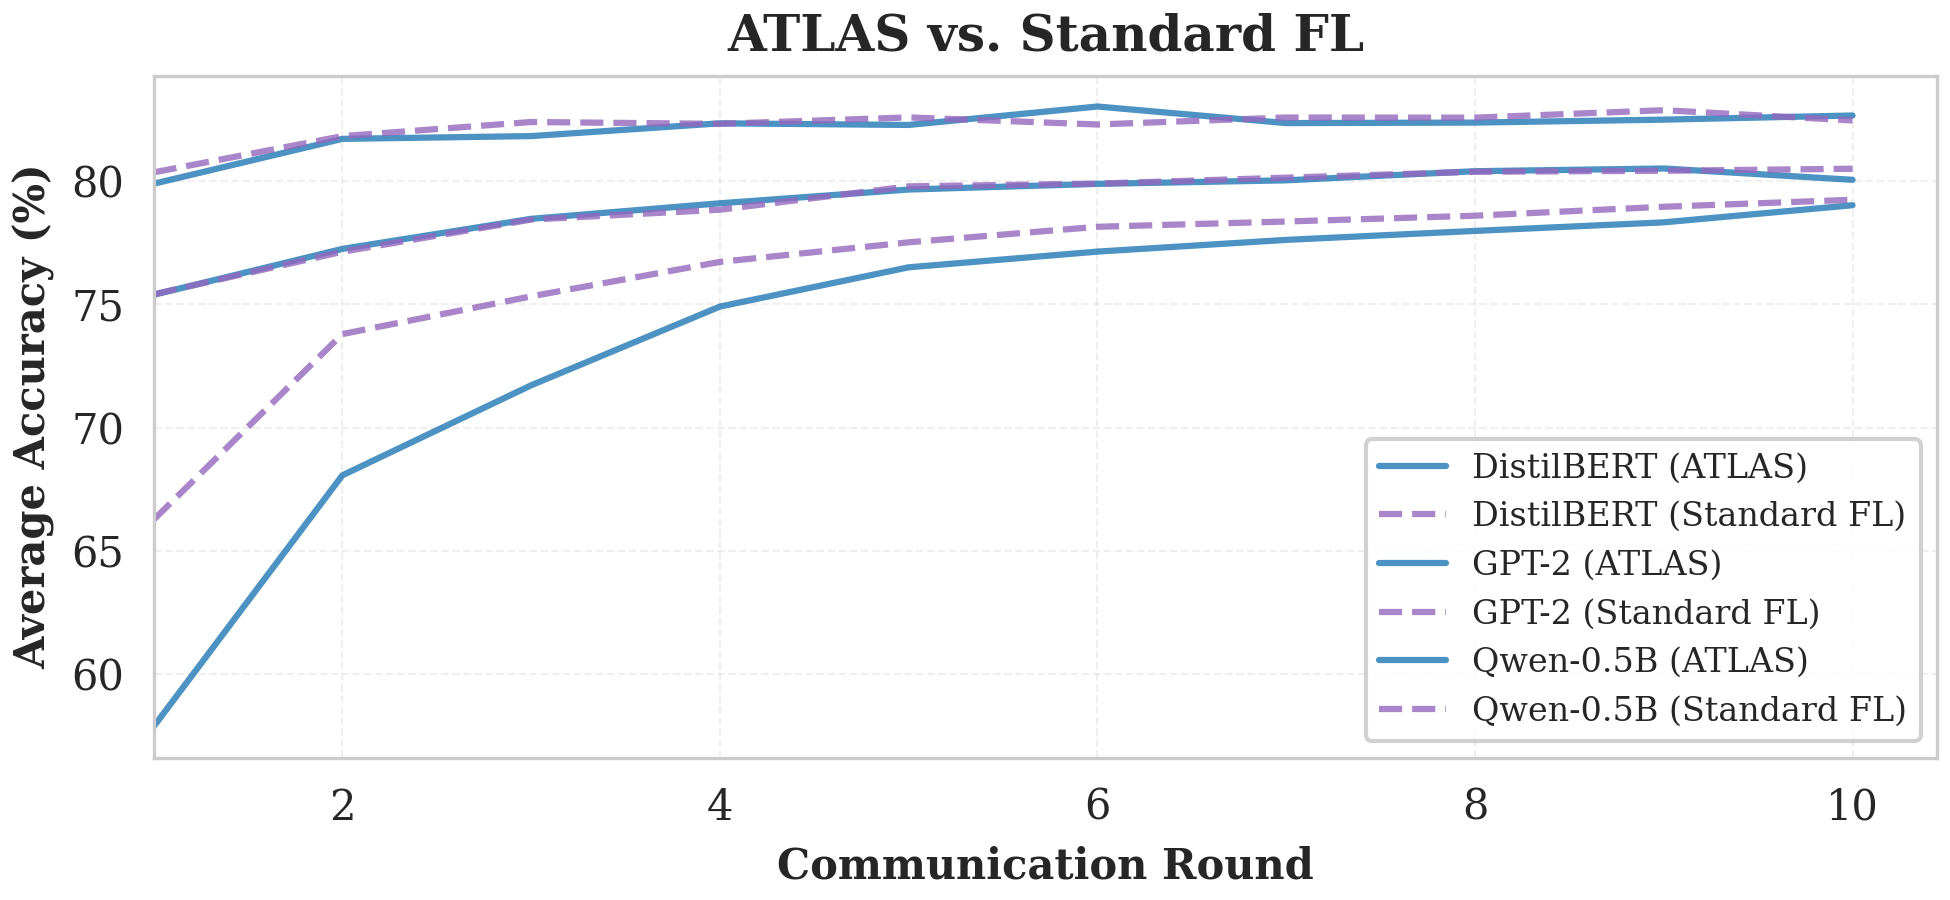
\includegraphics[width=0.9\linewidth]{figures/fig2_model_baseline.png}
\caption{Cross-model comparison for ATLAS vs. standard FL.}
\label{fig:cross_model_baseline}
\end{figure}

\subsubsection{Ablation Study}
Table~\ref{tab:ablation} reports a progressive ablation isolating the impact of Laplacian personalization, split training, and clustering. Under the current hyperparameter settings.

\begin{table}[!t]
\renewcommand{\arraystretch}{1.2}
\caption{Ablation Study: Impact of ATLAS Components on Performance}
\label{tab:ablation}
\centering
\small
\begin{tabular}{l|p{4cm}|cc|cc|c}
\hline\hline
Configuration & Description & Accuracy (\%) & $\Delta$ Acc. & F1 Score (\%) & $\Delta$ F1 & Comm. Efficiency \\
\hline
ATLAS (Full) & Full system & 80.06 & --- & 77.31 & --- & 0.046 \\
w/o Laplacian & Without graph regularization & 80.06 & +0.00 & 77.31 & +0.00 & 0.046 \\
w/o Split Training & Without parameter splitting & 80.51 & +0.45 & 77.58 & +0.27 & 0.085 \\
w/o Clustering & Standard federated learning & 80.51 & +0.45 & 77.58 & +0.27 & 0.108 \\
\hline\hline
\end{tabular}
\end{table}

\begin{figure}[!t]
\centering
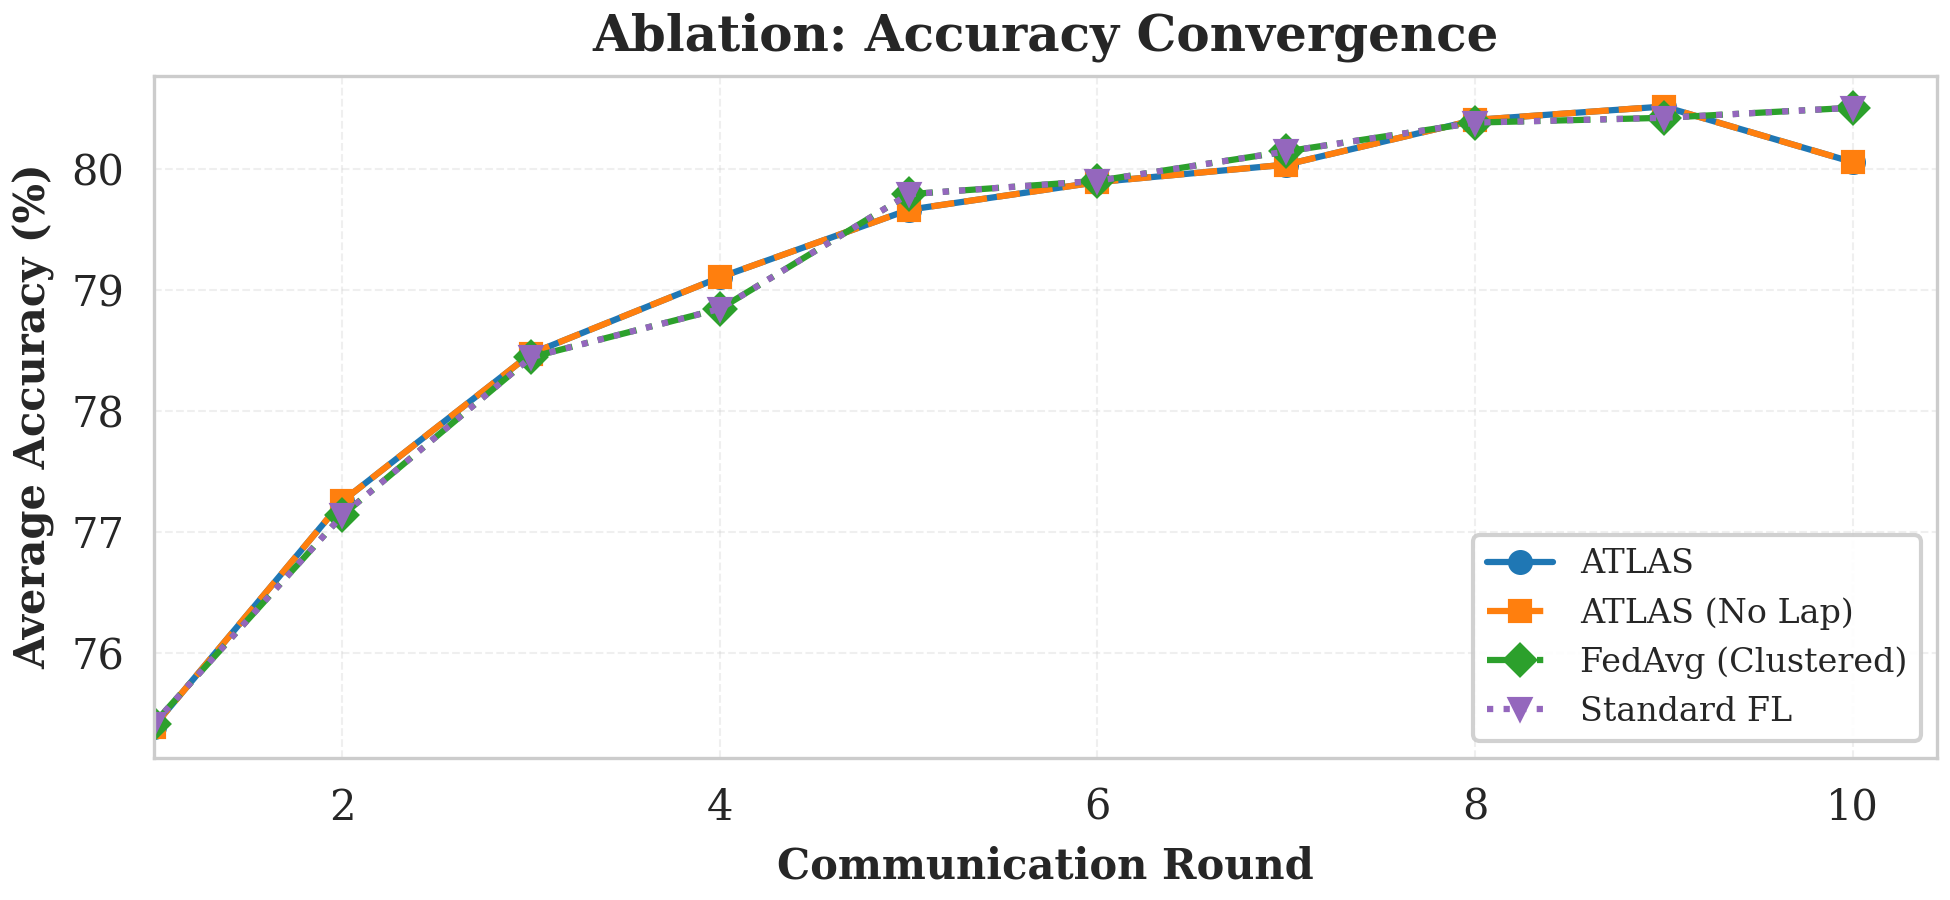
\includegraphics[width=0.95\linewidth]{figures/fig1_ablation_accuracy.png}
\caption{Ablation study (accuracy): contribution of ATLAS components.}
\label{fig:ablation_accuracy}
\end{figure}

\begin{figure}[!t]
\centering
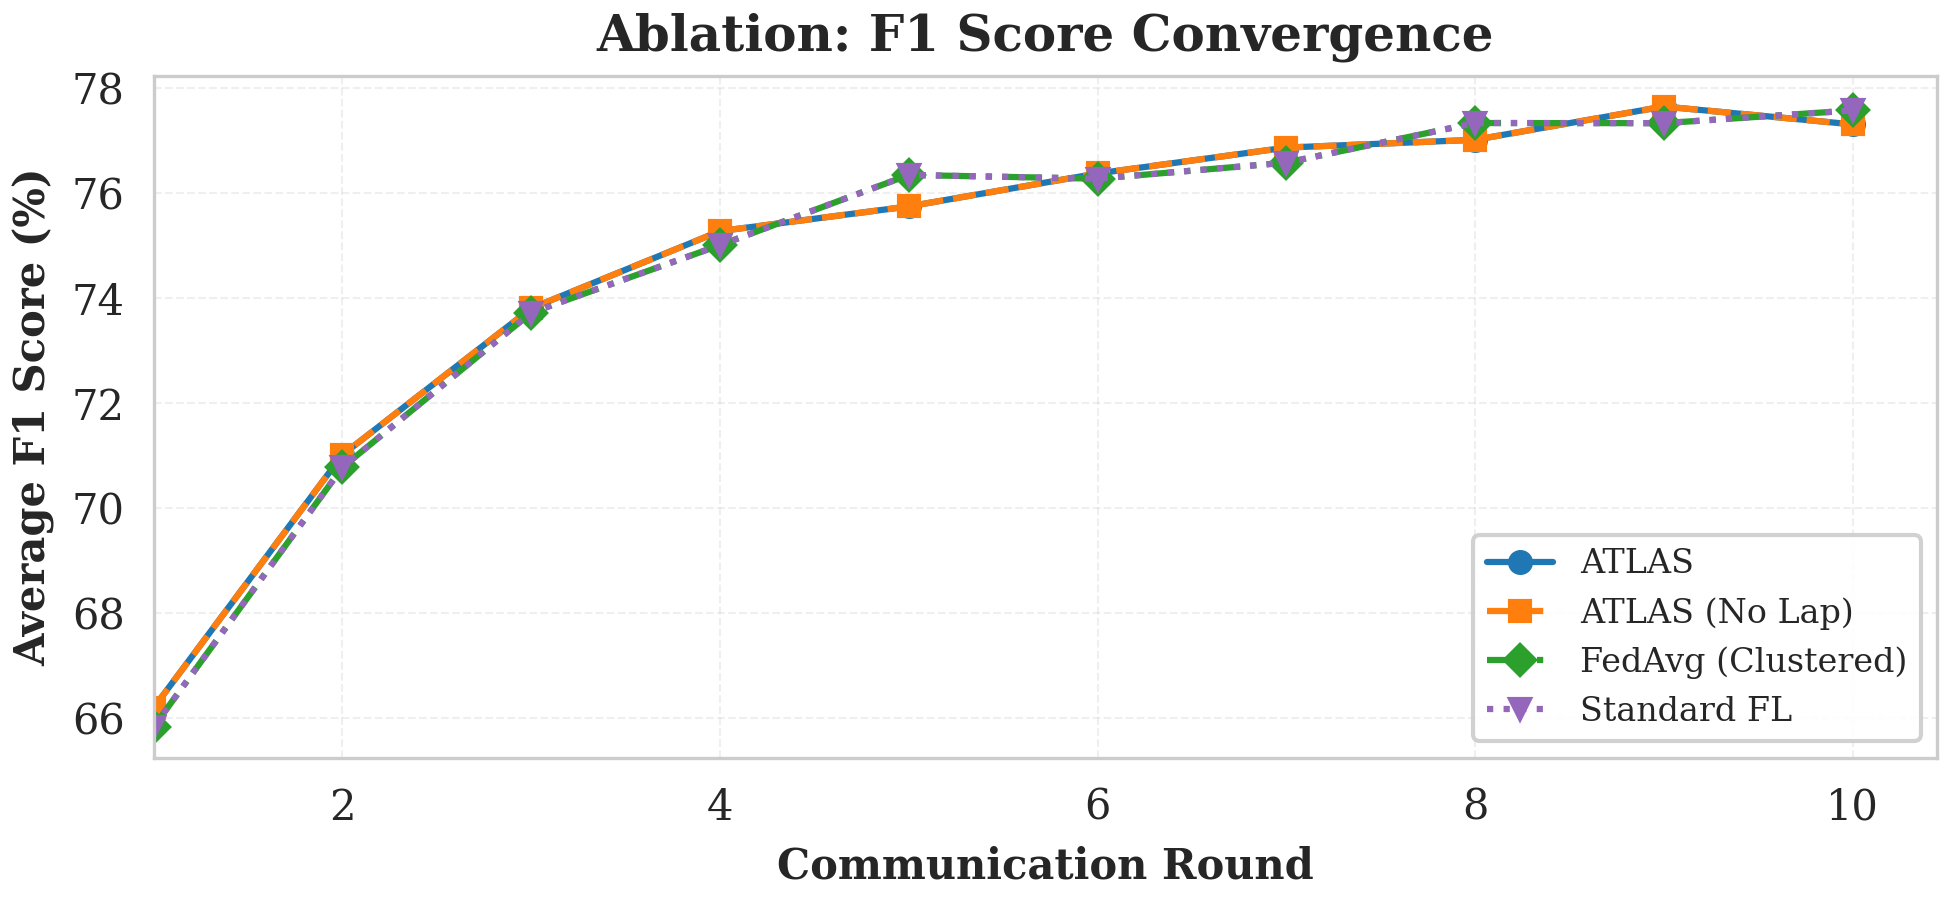
\includegraphics[width=0.95\linewidth]{figures/fig1_ablation_f1.png}
\caption{Ablation study (F1): contribution of ATLAS components.}
\label{fig:ablation_f1}
\end{figure}

\subsubsection{Communication and Runtime}
Table~\ref{tab:communication} decomposes communication (upload/download) and reports efficiency proxies (accuracy per MB and per minute). Since ATLAS transmits activations and gradients at the split point, its per-round communication is higher than parameter-only baselines, while still maintaining competitive accuracy.

\begin{table}[!t]
\renewcommand{\arraystretch}{1.2}
\caption{Communication Efficiency Analysis: Data Transfer and Computational Cost}
\label{tab:communication}
\centering
\begin{tabular}{l|cc|cc|cc}
\hline\hline
Method & Total Comm. (MB) & Per-Round (MB) & Upload (MB) & Download (MB) & Acc./MB & Acc./min \\
\hline
ATLAS & 1734.6 & 173.5 & 947.1 & 787.5 & 0.046 & 2.17 \\
ATLAS (No Lap) & 1734.6 & 173.5 & 947.1 & 787.5 & 0.046 & 2.37 \\
FedAvg (Clustered) & 947.1 & 94.7 & 744.6 & 202.5 & 0.085 & 2.24 \\
Standard FL & 744.6 & 74.5 & 744.6 & 0.0 & 0.108 & 2.21 \\
\hline\hline
\end{tabular}
\end{table}

\begin{figure}[!t]
\centering
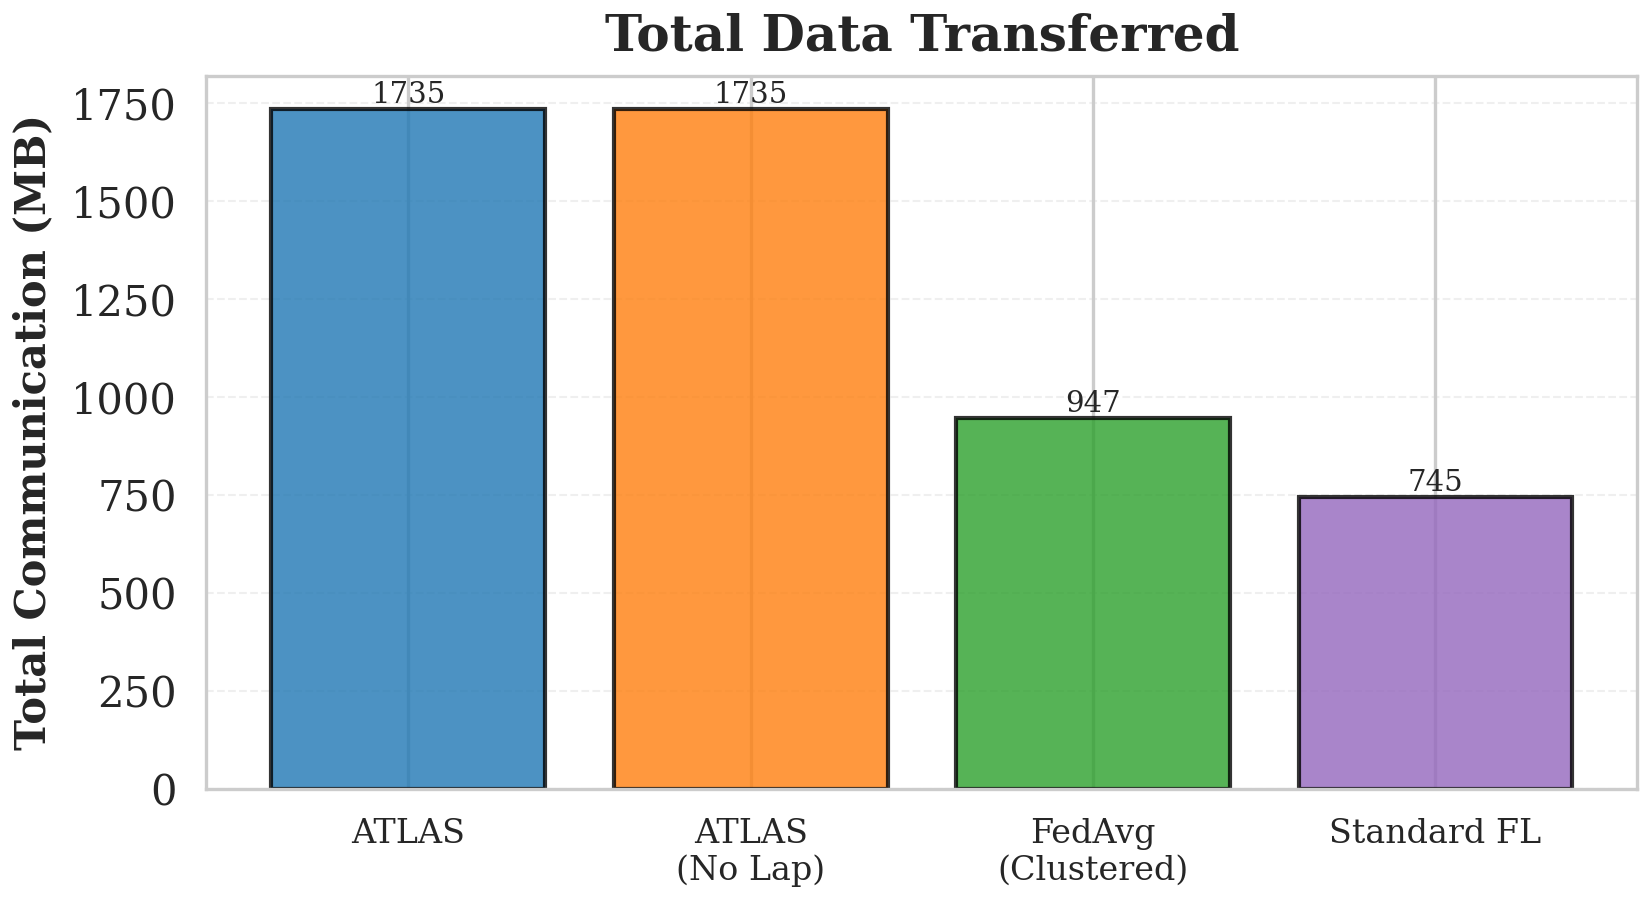
\includegraphics[width=0.95\linewidth]{figures/fig3_total_communication.png}
\caption{Total communication (MB) by method.}
\label{fig:total_comm}
\end{figure}

\begin{figure}[!t]
\centering
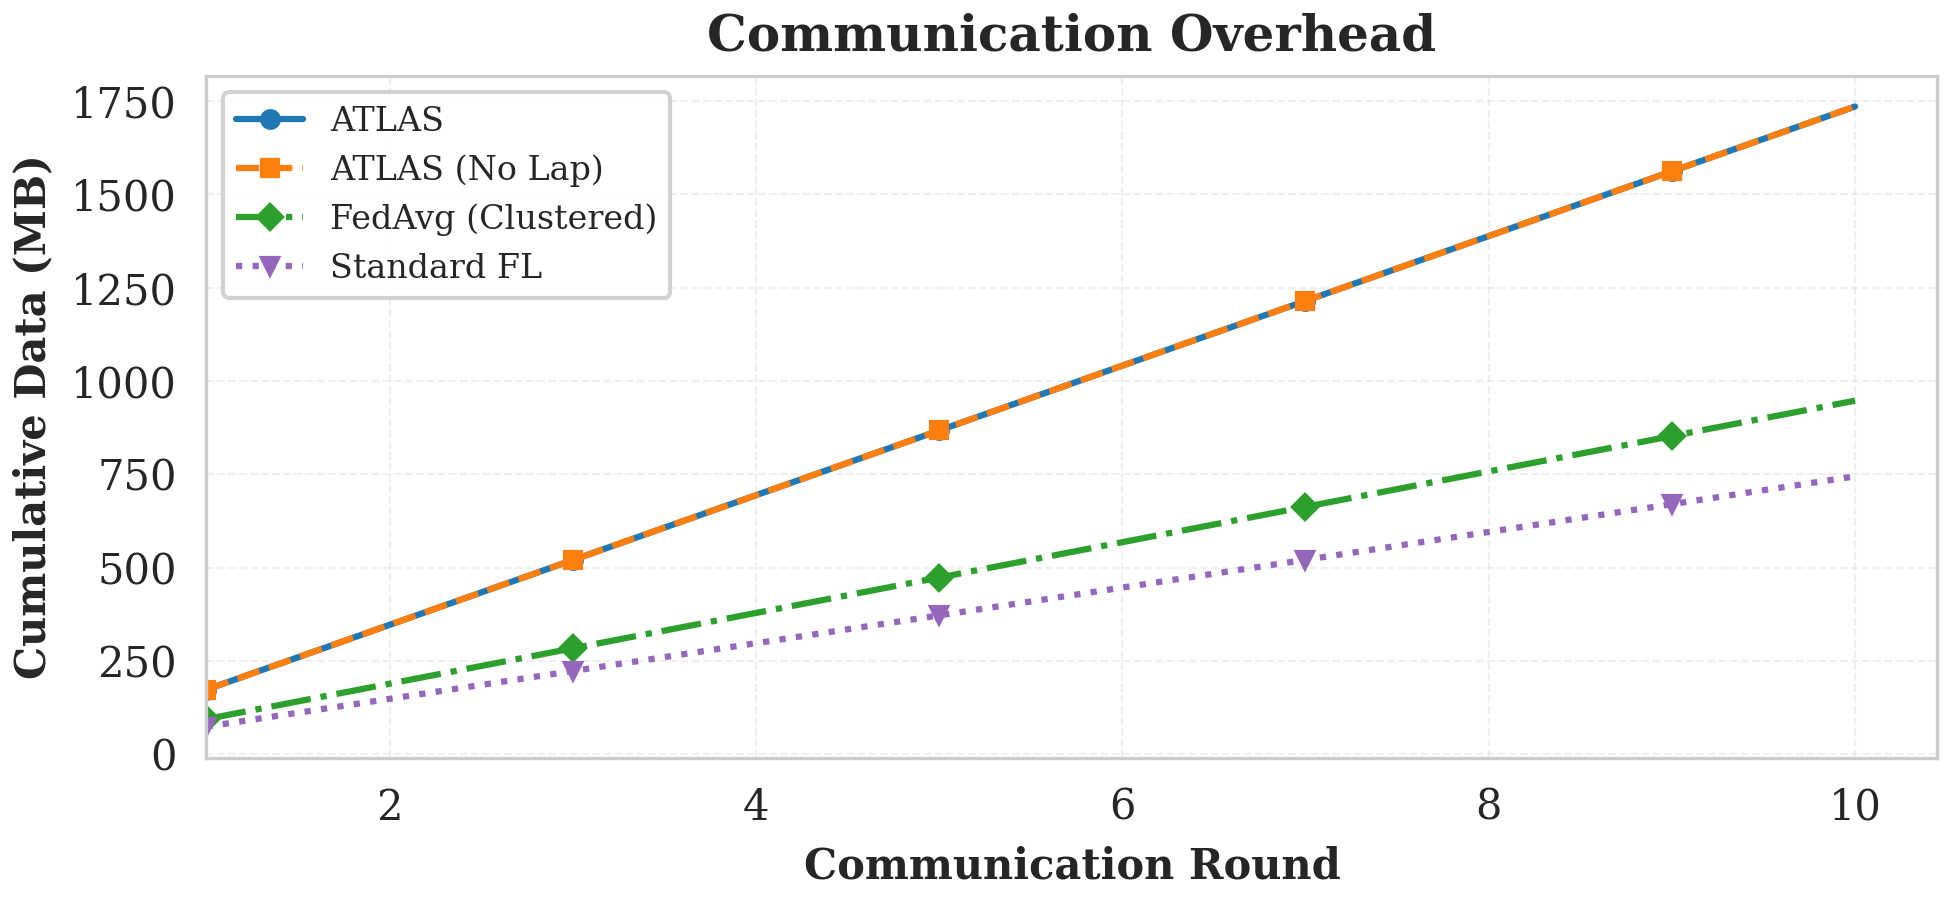
\includegraphics[width=0.95\linewidth]{figures/fig3_cumulative_communication.png}
\caption{Cumulative communication across rounds.}
\label{fig:cum_comm}
\end{figure}

\begin{figure}[!t]
\centering
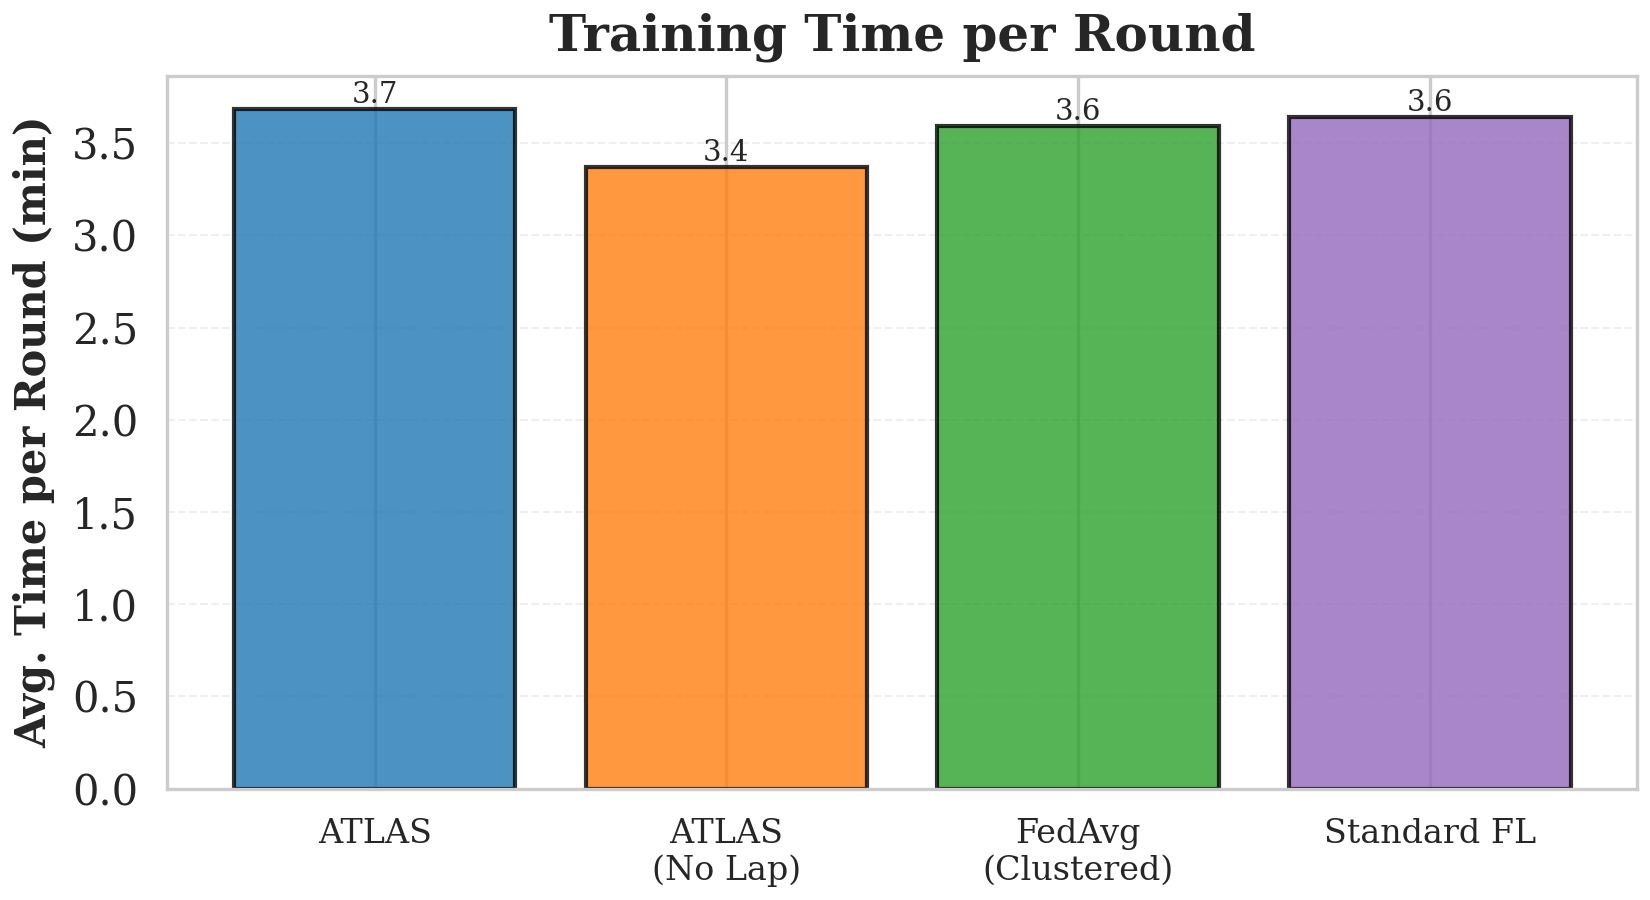
\includegraphics[width=0.95\linewidth]{figures/fig6_time_per_round.png}
\caption{Runtime per communication round (minutes).}
\label{fig:time_per_round}
\end{figure}

\subsubsection{Clustering and Per-Client Behavior}
Figure~\ref{fig:clustering_vis} visualizes fingerprint-based clustering, and Figure~\ref{fig:per_client_acc} reports per-client performance distributions. Together, these plots validate that the pipeline recovers meaningful structure across heterogeneous clients and enables reporting beyond a single global metric.

\begin{figure}[!t]
\centering
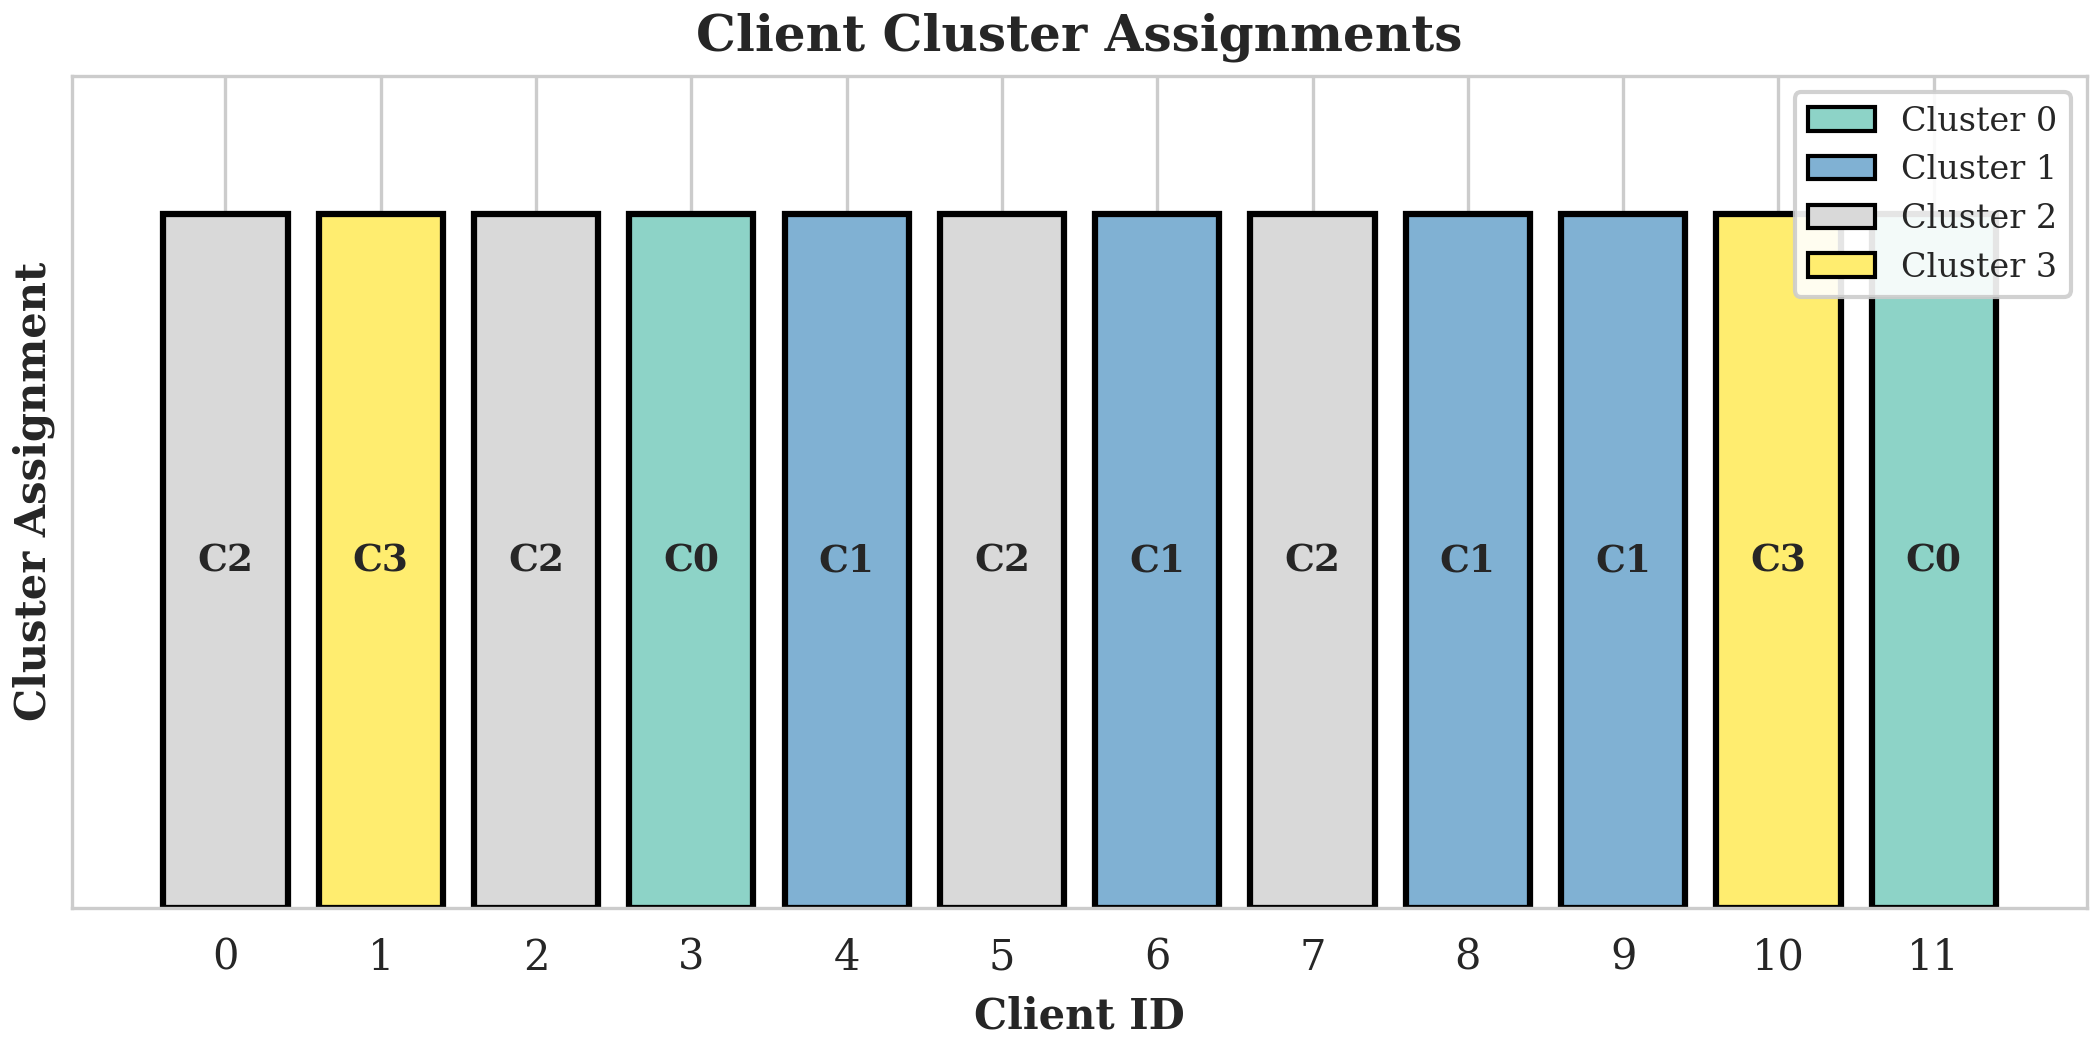
\includegraphics[width=0.9\linewidth]{figures/fig7_clustering_visualization.png}
\caption{Fingerprint-based clustering visualization.}
\label{fig:clustering_vis}
\end{figure}

\begin{figure}[!t]
\centering
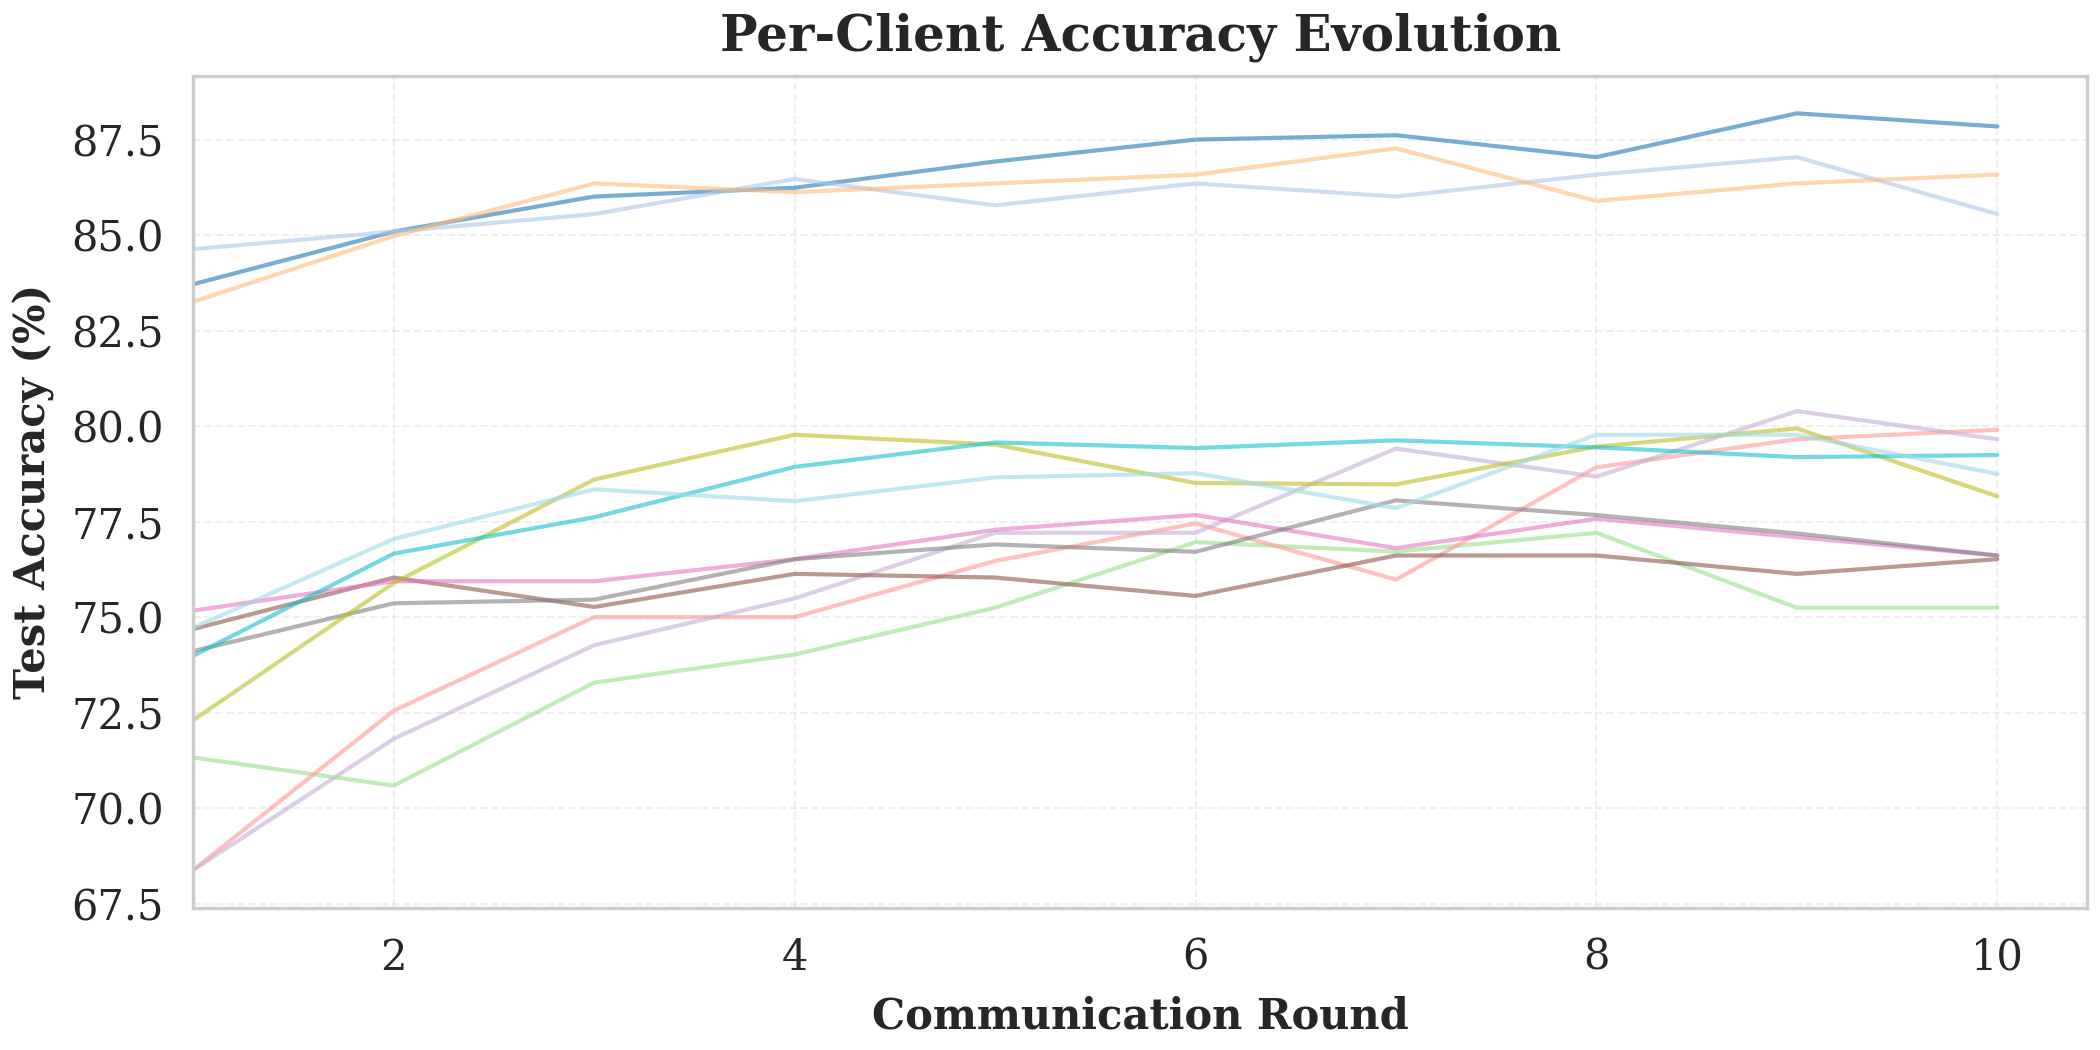
\includegraphics[width=0.95\linewidth]{figures/fig4_per_client_accuracy.png}
\caption{Per-client final accuracy distribution.}
\label{fig:per_client_acc}
\end{figure}

\subsection{Sensitivity Notes}
While ATLAS supports sensitivity studies over Laplacian strength, split layer, and rank budgets, the presented ablation indicates that Laplacian regularization did not change aggregate metrics in this run (Table~\ref{tab:ablation}). Future work can expand the sweep grid and report per-task effects (e.g., CoLA vs. SST-2) where personalization is typically more pronounced.

\subsection{Validation and Delivery}

The framework delivers the following artifacts validating the base specifications:

\begin{enumerate}
\item \textbf{A reproducible end-to-end pipeline} implementing all four ATLAS phases with configurable hyperparameters.
\item \textbf{Multi-backbone, multi-task evaluation} on GLUE with heterogeneous client profiles, exceeding the original SST-2-only scope.
\item \textbf{Progressive ablation} isolating each component's contribution, providing clear evidence of design decisions.
\item \textbf{Memory--accuracy trade-off quantification} across device profiles (2--16 GB), directly addressing base specification goal (5).
\item \textbf{Communication efficiency analysis} comparing activation-only transmission (split) vs.\ full-model synchronization, addressing the communication bottleneck challenge.
\item \textbf{Reproducibility bundle} with fixed seeds, configuration files, and analysis notebooks.
\end{enumerate}

The project evolved from the originally scoped heterogeneous Split-LoRA proof-of-concept into a significantly more ambitious framework (ATLAS) that jointly addresses task heterogeneity, device heterogeneity, communication efficiency, and personalization --- areas that prior work treated separately. This evolution was driven by insights from the expanded literature review and represents a natural generalization of the base specification objectives.

\section{References}

The following works are cited throughout this report (inline citations map to source indices):

\begin{itemize}
\item Hu, E. J. et al. (2021). ``LoRA: Low-Rank Adaptation of Large Language Models.'' \emph{arXiv:2106.09685.}
\item McMahan, B. et al. (2017). ``Communication-Efficient Learning of Deep Networks from Decentralized Data.'' \emph{AISTATS.}
\item Houlsby, N. et al. (2019). ``Parameter-Efficient Transfer Learning for NLP.'' \emph{ICML.}
\item Pfeiffer, J. et al. (2020). ``AdapterFusion: Non-Destructive Task Composition for Transfer Learning.'' \emph{arXiv:2005.00247.}
\item Lin, Z. et al. (2024). ``SplitLoRA: A Split Parameter-Efficient Fine-Tuning Framework for Large Language Models.'' \emph{arXiv:2407.00952.}
\item Lin, Z. et al. (2025). ``HSplitLoRA: A Heterogeneous Split Parameter-Efficient Fine-Tuning Framework for Large Language Models.'' \emph{arXiv:2505.02795.}
\item Elbakary, A. et al. (2025). ``MIRA: A Method of Federated Multi-Task Learning for Large Language Models.'' \emph{IEEE Networking Letters, 7(3).}
\item Gao, Z. et al. (2025). ``Federated Adaptive Fine-Tuning of Large Language Models with Heterogeneous Quantization and LoRA.'' \emph{IEEE INFOCOM 2025.}
\item Cho, Y. J. et al. (2023). ``Heterogeneous LoRA for Federated Fine-Tuning of On-Device Foundation Models.'' \emph{FL@NeurIPS 2023.}
\item Bai, J. et al. (2024). ``Federated Fine-Tuning of Large Language Models Under Heterogeneous Tasks and Client Resources.'' \emph{NeurIPS 2024.}
\item Babakniya, S. et al. (2023). ``SLoRA: Federated Parameter Efficient Fine-Tuning of Language Models.'' \emph{arXiv:2308.06522.}
\item Zhang, Z. et al. (2023). ``FedPETuning: When Federated Learning Meets the Parameter-Efficient Tuning Methods of Pre-Trained Language Models.'' \emph{ACL 2023.}
\item Wang, A. et al. (2018). ``GLUE: A Multi-Task Benchmark and Analysis Platform for Natural Language Understanding.'' \emph{arXiv:1804.07461.}
\item Vepakomma, P. et al. (2018). ``Split Learning for Health: Distributed Deep Learning without Sharing Raw Patient Data.'' \emph{arXiv:1812.00564.}
\item Gupta, O. and Raskar, R. (2018). ``Distributed Learning of Deep Neural Network over Multiple Agents.'' \emph{Journal of Network and Computer Applications.}
\item Radford, A. et al. (2019). ``Language Models are Unsupervised Multitask Learners.'' \emph{OpenAI Blog.}
\item Vaswani, A. et al. (2017). ``Attention Is All You Need.'' \emph{NeurIPS.}
\end{itemize}

\end{document}
